% !TeX spellcheck = en_US
\documentclass[french]{yLectureNote}

\title{Électromagnétisme 1 PS}
\subtitle{Physique}
\author{Paulhenry Saux}
\date{\today}
\yLanguage{Français}
%lionels.calmels@cemes.fr
\professor{F.Pettinari}
\usepackage{graphicx}%----pour mettre des images
\usepackage[utf8]{inputenc}%---encodage
\usepackage{geometry}%---pour modifier les tailles et mettre a4paper
%\usepackage{awesomebox}%---pour les boites d'exercices, de pbq et de croquis ---d\'esactiv\'e pour les TP de PC
\usepackage{tikz}%---pour deiffner + d\'ependance de chemfig
% \usepackage{tabularx}%---pour dimensionner automatiquement les tableaux avec variable X
\usepackage{awesomebox}%---Pour les boites info, danger et autres
\usepackage{menukeys}%---Pour deiffner les touches de Calculatrice
\usepackage{fancyhdr}%---pour les en-t\^ete personnalis\'ees
\usepackage{blindtext}%---pour les liens
\usepackage{hyperref}%---pour les liens (\`a mettre en dernier)
\usepackage{caption}%---pour la francisation de la l\'egende table vers Tableau
\usepackage{pifont}
\usepackage{array}%---pour les tableaux
\usepackage{lipsum}
\usepackage{yFlatTable}
\usepackage{multicol}
\newcommand{\Lim}[1]{\lim\limits_{\substack{#1}}\:}
\renewcommand{\vec}{\overrightarrow}
\newcommand{\N}[0]{\mathbb{N}}
\newcommand{\dd}{\mathrm{d}}
\newcommand{\norm}[1]{||\vec{#1}||}
\newcommand{\fo}{\psi(\vec{r},t)}
\newcommand{\foe}{\psi(\vec{r},t)\*}
\newcommand{\HH}{\hat{H}}
\newcommand{\hb}{\hbar}
\newcommand{\lap}{\nabla^2}
\newcommand{\lapcc}{\frac{\partial^2 }{\partial x^2}+\frac{\partial^2 }{\partial y^2}+\frac{\partial^2 }{\partial z^2}}
\newcommand{\E}{\vec{E}(M)}
\newcommand{\B}{\vec{B}(M)}
\newcommand{\V}{V(M)}
\newcommand{\er}{\vec{e_{\rho}}}
\newcommand{\ep}{\vec{e_{\varphi}}}
\newcommand{\pip}{\pi^+}
\newcommand{\pim}{\pi^-}
\newcommand{\mv}{\mathcal{V}}
\begin{document}
\setcounter{chapter}{5}
\chapter{Distributions de courant électrique}
\section{Distribution voumique et densité de courant}
\subsection{Densité volumique de courant}
\subsubsection{Mise en situation}
On relie les faces du cylindre à des potentiels de courant à l'aide de 2 générateurs de tension.

Comme \(V_2\neq V_1\), il existe un champ électrique orienté dans le sens des potentiels décroissants dans le conducteur, orthogonal aux surfaces équipotentielles, parallèles aux faces d'entrée et sortie.

Comme les électrons ont un charge négative, la force exercée sera de sens opposé au champ.
\subsubsection{Régime permanent}
Les électrons atteignent une vitesse de dérive \(\vec{v}\) opposée à \(\E\), qui dépend de E, du matériau (densité de défaut qui ralentissent les électrons) et de la température (vibration des atomes)
\subsubsection{Densité volumique de courant}
\begin{definition}[DVC]
\[\vec{j} = \rho_c\vec{v} = -ne\vec{v}\] avec n le nombre d’électrons. Elle est opposée à \(\vec{v}\).
\end{definition}


Le lien entre ces quantités dépend du matériau considéré, de sa qualité cristalline, et des défauts atomiques contenus à l'échelle du nanomètre et de la température.

\[\vec{j} = \gamma \vec{E}\] avec \(\gamma\) la conductivité électrique du matériau. C'est la loi d'Ohm locale.

Moins il y a de défauts, plus \(\gamma\) sera grand.
\subsection{Intensité du courant électrique}
Soit \(\vec{n}\) le vecteur normal à une section\marginInfo{C'est pourquoi les 2 vecteurs ne sont pas colinéaires.} quelconque et \(\vec{j}\) le vecteur densité volumique du courant.

On peut définir l'intensité du courant électrique dans ce câble comme
\begin{definition}[Intensité du courant électrique]
\[I = \iint_{S}\vec{j}\cdot \vec{n}\dd S\] avec S la section étudiée
\end{definition}
\warningInfo{Remarques}{
Le choix du sens de \(\vec{n}\) est arbitraire et sans importance, cependant il détermine le signe de I, mais cela ne change pas les propriétés physiques calculées. En effet, le fait de choisir un sens impose simplement la flèche indiquant le sens de I sur le câble. Or, changer de sens ne change rien physiquement. Si on change le sens, on change aussi le signe : cela correspond à la m\^eme situation.
}
\criticalInfo{Choix de la section}{L'avantage d'écrire I sous cette forme : Le résultat ne dépend pas de la section choisie.}
\subsection{Loi d'Ohm Intégrale}
On considère le m\^eme câble, avec une \emph{densité volumique de courant uniforme} avec la face d'entrée portée au potentiel \(V_1\) et la face de sortie à \(V_2< V_1\). Ce sont des surfaces équipotentielles. On choisit d'orienter \(\vec{n}\) dans le sens  des potentiels décroissants.

\[I = \iint \vec{j}\cdot \vec{n}\dd S = \iint \gamma E\vec{e_z}\cdot \vec{e_z}\dd S = \gamma ES\]

On applique l'équation locale entre \(V\) et \(\E\) :
\begin{flalign*}
V(M_2)-V(M_1) &= - \int E\vec{e_z}\cdot \dd z \vec{e_z}\\
&= -E\int_{z_1}^{z_2}\dd z\\
&= -E(z_2-z_1)\\
&=-E\cdot l\\
V_1-V_2 &= El
\end{flalign*}

On en déduit la loi d'Ohm intégrale :
\begin{theorem}[Loi d'Oh intégrale]
\(V_1-V_2 = \frac{lI}{\gamma S}\)
\end{theorem}

\subsection{Dimensions}
On sait que \(I = \iint \vec{j}\vec{n}\dd S \Rightarrow I = [j]L^2 \Rightarrow [j] = \frac{I}{L^2}\). Ce ne sont pas des volumes. On étudie le courant dans un conducteur 3D.
\section{Distributions surfaciques de courant}
On considère un ruban métallique, avec \(n_s\) la densité surfacique d'électrons de conduction, \(\vec{j_S}\) la densité surfacique de courant dans le conducteur 2D qui vaut \(\vec{j_s} = -n_S e\vec{v}\). Soit C une courbe coupant le ruban, M un point sur C, \(\vec{n}\) la normale à C.

On a \(I = \int_C \vec{j}\cdot \vec{n}\dd l\)
\section{Distributions linéiques de courant}
On étudie un ensemble de fil parcourue par des intensité données.
Soit \(I_i\) les intensités algébriques.
\section{Éléments de symétrie d'une distribution de courant}
\subsection{Plan \(\pip\)}
Soient \(M_1(x,y,z), M_2(x,y,-z)\) symétriques l'un de l'autre // au plan (Oxy). C'est un plan \(\pip\) si les 2 vecteurs sont symétriques par rapport au plan.

Il y a aussi le plan médiateur à 2 distributions linéiques de m\^eme intensité.
\subsection{Plan \(\pim\)}
C'est la m\^eme définition sauf que \(\vec{j}\) serait opposée (sens différent) à ce qu'il serait si on avait un plan \(\pim\).

C'est le cas des plans orthogonaux à l'axe.
\section{Invariance d'une distribution de courant}
Si \(\vec{j}\) est constant \(\forall z\), alors la distribution de courant est invariante par toute translation parallèle à l'axe Oz. De m\^eme pour la coordonnée \(\varphi\), la distribution est invariante par translation autour de Oz.
\chapter{Champ magnétique : Biot et Savart}
\section{Champ \(\vec{B}(M)\) créé par un fil}
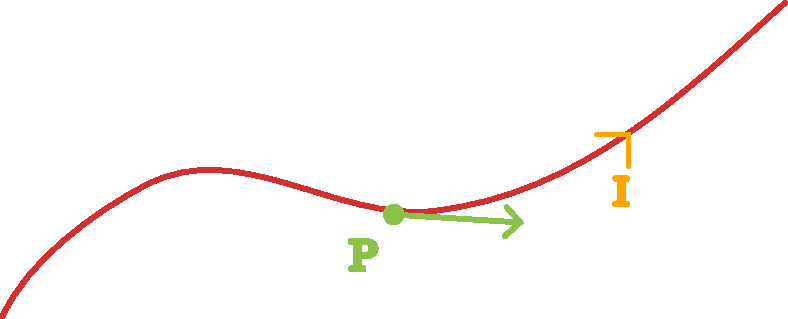
\includegraphics[scale=0.5]{fil}

On suppose un champ \(\B\) crée par un fil d'épaisseur négligeable parcourue par un courant électrique d'intensité I\marginCheck[Rappel]{I est algébrique}. On note P un point du fil électrique, et \(\vec{\dd l(P)}\) le long du fil électrique, orienté dans le sens du courant au point P.

M est le point pour lequel on veut calculer le champ magnétique crée par ce courant.

On admettra que le fil  de longueur élémentaire \(\dd l(P)\) parcourue par le courant d'intensité I crée en M le champ magnétique élémentaire :
\begin{theorem}[Champ magnétique élémentaire d'un fil]
 \[\dd B(M) = \frac{\mu_0}{4\pi} \frac{I \vec{\dd l}(P)\wedge \vec{PM}}{\norm{PM}^2}\] avec \(\mu_0 = 4\pi \cdot 10^{-7}\)
\end{theorem}
On remarque \(\norm{\dd \B}\) décroît en \(\frac{1}{\norm{PM}^2}\)

La dimension de \(\vec{\dd B(M)}\) est \(\frac{[\mu_0]I}{L}\).

On n' a plus qu'à faire l'intégrale :
\begin{theorem}[Loi de Biot et Savat]
 \[\B = \int_{P\in F} \frac{\mu_0}{4\pi} \frac{I\vec{\dd l}(P)\wedge \vec{PM}}{\norm{PM}^2}\]
\end{theorem}
% L'intégrale porte sur la coordonnée du point P permettant de repérer sa position sur le fil.
\section{Distribution surfacique}
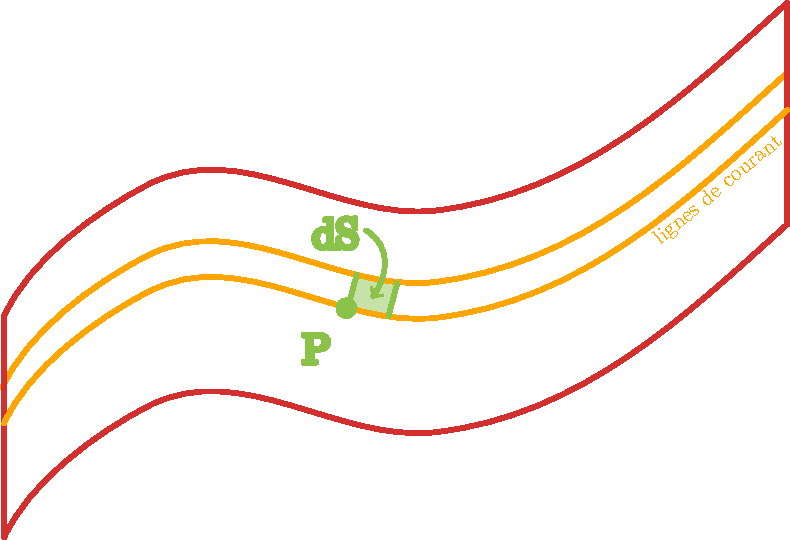
\includegraphics[scale=0.5]{surface}

On considère un ruban parcouru par une densité surfacique de courant. P est un point sur le ruban. On note \(\dd S(P)\) située au point P et délimitée par des lignes de courant. \(j_s(P)\) est la densité surfacique de courant au point P. Sur \(\dd S(P)\), \(j_s\) est considéré uniforme sur la surface.

Le champ magnétique élémentaire crée en M  est \[\dd \B = \frac{\mu_0}{4\pi}\frac{\dd S \vec{j_s}(P)\wedge \vec{PM}}{\norm{PM}^3}\]

On n' a plus qu'à intégrer : \[\iint_{P\in S} \frac{\mu_0}{4\pi}\frac{\dd S \vec{j_s}(P)\wedge \vec{PM}}{\norm{PM}^3}\]
\section{Distribution volumique de courant}
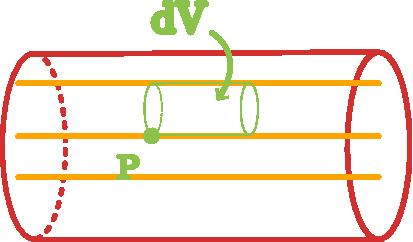
\includegraphics[scale=0.7]{volume}

De la m\^eme façon, P est un point dans le câble, \(\vec{j_p}\) la densité volumique de courant au point P. \(\dd \mv\) est le volume élémentaire délimité latéralement par des lignes de courant. On obtient \[\B = \iiint_{P\in \mv} \frac{\mu_0}{4\pi}\frac{\dd \mv \vec{j}(P)\wedge \vec{PM}}{\norm{PM}^3}\]

\section{Fil infiniment long}
La distribution de courant est à symétrie cylindrique autour du fil d'axe Oz, M est repéré par ses coordonnées cylindriques dans la base cylindrique locale. La position de P sur le fil est repérée par \(z_p\) et on  a \(\vec{\dd l}(P) = \dd z_p \vec{e_z}\).

On écrit \(\vec{PM} = -z_p\vec{e_z}+ (\rho \er+z\vec{e_z})\)

Il y a invariance par translation selon \(e_z\) du courant. Pour simplifier, on peut faire le calcul en mettant M dans le plan \(Oxy\).  On a donc \(\vec{PM} = -z_p\vec{e_z}+\rho \er\).

On écrit :
\explanation{1}{On utilise la primitive vue en TD et on l'évalue aux limites en \(\pm \infty\)}
\begin{flalign*}
\dd \B &= \frac{\mu_0}{4\pi} \frac{I\dd z_p \vec{e_z}\wedge (-z_p\vec{e_z}+\rho \er)}{(z_p^2+\rho^2)^{3/2}}\\
&=  \frac{\mu_0}{4\pi} \frac{\rho I \dd s_p \ep}{(z_p^2+\rho^2)^{3/2}}\\
&\Rightarrow \B = \int^{\infty}_{-\infty} \dd \B\\
& = \frac{\mu_0 I\rho}{4\pi}\ep \int \frac{\dd z_p}{(z_p^2+\rho^2)^{3/2}}\\
&= \frac{\mu_0 I\rho}{4\pi}\ep \frac{2}{\rho^2}\explain{1}{right}{0}{0.5}{} \\
&= \frac{\mu_0 I\rho}{2\pi \rho}\ep
\end{flalign*}
\begin{proposition}[Champ crée par un fil infiniment long]
\[\vec{B}(M) = \frac{\mu_0 I\rho}{2\pi \rho}\vec{\vec{e_{\varphi}}}\]
\end{proposition}

Le champ est toujours selon \(\ep\), donc orthoradial et les lignes de champ sont circulaires. Si I est négatif, les lignes sont orientées dans le sens opposé.
\section{Spire circulaire}
On cherche maintenant le champ crée par une spire circulaire crée en un point M placé sur l'axe de la spire.

Compte tenu des symétries autour de  l'axe de la spire, on écrit P avec ses coordonnées cylindriques dans la base locale. On a \(\dd l(P) = R\dd \varphi_p \vec{e_{\varphi_P}} \). De plus, \(\vec{PM} = - R\vec{e_{\varphi_P}}+z\vec{e_z})\). En injectant dans la loi de Biot et Savat :
\begin{flalign*}
\dd \B &= \frac{\mu_0}{4\pi}  \frac{IR \dd \varphi_P \vec{\varphi_P}(-R \vec{e_{\varphi_P}}+z\vec{e_z})}{(R^2+z^2)^{3/2}}\\
&= \frac{\mu_0 IR \dd \varphi_{P}}{4\pi (R^2+z^2)^{3/2}}(R\vec{e_z}+z\vec{e_{\rho_P}})
\end{flalign*}
On remarque qu'il y a 2 composantes, et non seulement une composante selon \(\vec{e_z}\) !
On voit géométriquement que 2 point diamétralement opposés forment une somme de db dont la composante selon \(\er\) s'annule.


\includegraphics[scale=0.5]{symetrie}

Donc on peut garder que la composante selon \(\vec{e_z}\) pour le calcul intégral.

On a donc \[\B = \frac{\mu_0IR^2}{2(R^2+z^2)^{3/2}}\vec{e_z}\]

On remarque que cela tend vers 0 en \(z^{-3}\). De plus, la fonction est paire car \(z^2\).
\checkInfo{Remarque : Autre expression de B}{On a \(\B = \frac{\mu_0 I}{2R}\sin^3(\alpha)\vec{e_z}\) avec \(\alpha\) l'angle sous lequel on voit la spire depuis M. En effet, \(\sin(\alpha) = \frac{R}{(R^2+z^2)^{1/2}}\)

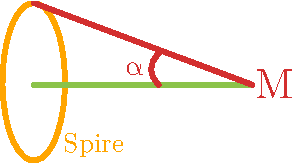
\includegraphics[scale=0.5]{spire}
}

\chapter{Propriétés de B}
\section{Théorème de superposition}
Le champ magnétique crée par un ensemble de distribution de courant vaut la somme de tout ces champs  crées par une distribution.
\section{Direction de B}
Vérifie les propriétés du produit vectoriel
\section{Conséquence des symétries de la Distribution de courant}
\subsection{Direction de \(\B\) en un point appartenant à un \(\pip\)}
 \end{document}
